\section{APR Analyses: Dynamic, Policy-Relative Teachers}
\label{sec:apr-analysis}

APR addresses a moving-target problem.  A trajectory that is a useful local
teacher for the current policy can become redundant after refinement, while a
previously distant candidate can enter the policy's compatible neighborhood.
The relevant question is therefore not whether additional optimization steps
help, but whether rebuilding and re-auditing the teacher set provides useful
targets while retaining already safe behavior.

\subsection{Round-wise behavior and protected components}
\label{sec:apr-rounds}

The main paper reports a monotonic sequence of 91.10, 91.21, 91.37, and 91.45
PDMS from Round 0 through Round 3, corresponding to gains of $+0.11$, $+0.16$,
and $+0.08$.  In the stage ablation, adding APR to the PC-MTS+FF-PGRPO policy
raises PDMS from 91.1 to 91.4 and EP from 86.0 to 86.7, while the displayed NC,
DAC, TTC, and comfort values remain 98.5, 98.0, 96.0, and 100, respectively.
This pattern is aligned with APR's design: local teacher updates increase
progress without visible regression in the protected components at the
reported precision.

Each round value is a reported checkpoint summary; its run/seed aggregation is
not stated.  No across-seed
standard deviation is available, and the 0.08--0.16 point increments are not
claimed to be independently significant.  Moreover, the archived experiment
history contains accepted and rejected branches rather than a single complete
three-round hash chain; the four values above are therefore treated as the
paper's round-level summary, not as permission to infer missing intermediate
measurements.

\begin{table}[t]
\centering
\small
\caption{Paper-reported NAVSIM v1 APR progression under single-trajectory inference. Higher is better. Run/seed aggregation is not stated and no training-seed confidence interval is available.}
\label{tab:apr_rounds}
\resizebox{\linewidth}{!}{%
\begin{tabular}{lcccc}
\toprule
round & pdms & gain\_points & evidence & runs \\
\midrule
0 & 91.1 & 0.0 & paper reported & reported point; run/seed aggregation not stated \\
1 & 91.21 & 0.11 & paper reported & reported point; run/seed aggregation not stated \\
2 & 91.37 & 0.16 & paper reported & reported point; run/seed aggregation not stated \\
3 & 91.45 & 0.08 & paper reported / final score scene-reproduced & reported point + 12138 final scenes; run aggregation not stated \\
\bottomrule
\end{tabular}%
}
\end{table}


\begin{figure}[t]
  \centering
  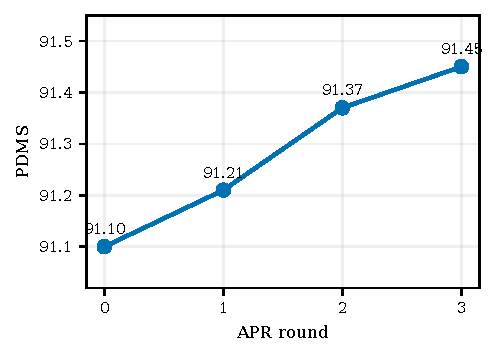
\includegraphics[width=\linewidth]{figures/generated/apr_rounds.pdf}
  \caption{Paper-reported NAVSIM v1 progression across APR rounds.  The final
  point is reproduced at scene level, but the small round increments are from
  one reported sequence and carry no across-seed error bar.}
  \label{fig:apr-rounds}
\end{figure}

\subsection{Teacher audit and post-interpolation evaluation}
\label{sec:apr-teacher-audit}

One traceable APR teacher-construction pass starts from 39,261 strict external
trajectories: 25,402 (64.7\%) from one driving-policy source and 13,859
(35.3\%) from a second source.  After interpolation with coefficient 0.25 and
exact re-evaluation, 28,910 targets remain, an acceptance rate of 73.6\%; the
remaining 10,351 are rejected.  These counts are from one audited navtrain
construction pass and are not presented as the source proportions of every
APR round.  They nevertheless establish an important operational fact:
interpolation is followed by evaluator-based admission, and the check is
non-vacuous---more than one quarter of the pre-audit union does not enter the
distillation set.

\begin{table}[t]
\centering
\small
\caption{Audited APR teacher-pool construction on NAVSIM navtrain. Counts are from one archived teacher audit; the 28,910 accepted teachers follow interpolation and exact re-evaluation. Higher acceptance is not inherently better because guards constrain quality.}
\label{tab:apr_teacher_pool}
\resizebox{\linewidth}{!}{%
\begin{tabular}{lcccc}
\toprule
step & source & count & acceptance\_definition & evidence \\
\midrule
source selection & DriVor & 25402 & source-specific strict candidates & archived APR runbook \\
source selection & DiffusionDriveV2 & 13859 & source-specific strict candidates & archived APR runbook \\
strict union & merged sources & 39261 & feasible and component-protected before interpolation & deterministic sum of audited source counts \\
post-interpolation audit & accepted teachers & 28910 & alpha 0.25 then exact re-evaluation & archived APR runbook \\
\bottomrule
\end{tabular}%
}
\end{table}


Teacher status is defined relative to the current policy.  A candidate is
\emph{accepted} when its evaluated local target is feasible, exceeds the
current single prediction by the required margin, preserves protected
metrics, and stays inside the current rollout neighborhood.  An accepted
teacher becomes \emph{expired} if it fails those tests after the policy is
updated.  A previously rejected candidate is \emph{newly activated} if it
passes after the rollout bank and current prediction are regenerated.  These
definitions prevent lifecycle counts from being conflated with raw pool size.

The interpolation search is descending: larger moves are evaluated first and
the first admissible move is retained.  Every accepted target stores the
teacher, current prediction, interpolation coefficient, post-interpolation
score, protected-metric deltas, compatibility distance, and evaluator hash.
No-interpolation and no-post-evaluation controls remove different safeguards:
the former jumps directly to the teacher, whereas the latter retains a local
trajectory without verifying that interpolation preserved feasibility.

\subsection{Step-matched controls}
\label{sec:apr-controls}

The release defines eight variants from the same Round-0 checkpoint and
matches the total number of optimizer updates: extra training on the existing
mixture, one-shot distillation, repeated use of a fixed teacher set, dynamic
teachers, dynamic teachers without interpolation, without post-interpolation
re-evaluation, without policy retention, and full APR.  The dynamic-teacher
and full-APR variants rebuild predictions, rollout banks, and teacher audits at
the same three round boundaries reported in the paper.  The fixed-teacher
variant repeats the Round-1 set without re-ranking it; the extra-training
control receives the same update count but no new teacher target.  This design
separates four possible explanations: more updates, teacher supervision in
general, teacher-set rebuilding, and the interpolation/retention safeguards.

For every round, the required report contains PDMS and all components,
regressed scenes, new failures, accepted/expired/newly activated teachers,
mean and median verified teacher advantage, interpolation-coefficient
distribution, and scene coverage.  A checkpoint is promoted only if its
single-trajectory aggregate score improves and protected metrics pass the
same non-regression audit; otherwise the previous checkpoint remains the
dynamic anchor.  Training ends after three promoted rounds or when no audited
local target remains.  These controls are configured but not represented as
measured results in this supplement, because running them would require new
training.

Optional task-vector consolidation is kept separate from teacher discovery.
The implementation can mask low-salience coordinates, require directional
agreement, bound each branch norm and the total displacement from the current
anchor, and then evaluate the merged checkpoint.  The best-branch, simple
average, task-arithmetic, and TIES-style controls are required before assigning
an independent gain to merging~\cite{taskarithmetic2023,ties2023}.  In the
absence of a stable, step-matched gain, merging should be read as a conservative
checkpoint-consolidation detail, not as the source of APR's teacher lifecycle.

The present evidence therefore supports two bounded statements: the reported
APR rounds are monotonic and preserve the displayed safety/compliance metrics,
and an audited construction pass materially filters proposed local targets
after re-evaluation.  The step-matched variants above are the necessary test
for the stronger causal claim that dynamic rebuilding, rather than additional
training alone, explains the full increment.

\begin{table}[t]
\centering
\small
\caption{APR fixed-teacher diagnostic on NAVSIM v1. The archived fixed-set continuation decreases from its 91.2766 anchor, whereas the 91.45 endpoint is the paper's compressed dynamic-round report; the rows are diagnostic rather than a step-matched causal ablation.}
\label{tab:apr_fixed_teacher}
\resizebox{\linewidth}{!}{%
\begin{tabular}{lccc}
\toprule
policy\_or\_epoch & pdms & interpretation & evidence \\
\midrule
dynamic-teacher anchor & 91.2766 & accepted dynamic-teacher checkpoint & archived APR runbook \\
fixed-set continuation epoch 0 & 91.2526 & below dynamic-teacher anchor & archived APR runbook \\
fixed-set continuation epoch 1 & 91.2311 & further below dynamic-teacher anchor & archived APR runbook \\
paper APR round 3 & 91.45 & compressed round-level paper report & paper reported \\
\bottomrule
\end{tabular}%
}
\end{table}

